\clearpage
\section{Named Entity Recognition}
\label{sec:ner}
Named entity recognition is the process of automatically identifying and classifying named entities in a text. This can include identifying and categorizing named entities such as people, organizations, locations, and so on. \\
NER systems might be used to automatically extract information from a large collection of documents, such as identifying all mentions of specific named entities or analyzing the relationships between different named entities. \\

\subsection{Weak labeling}
During the creation of the ticket, we tried to automatically save also the entities of the ticket. With entities, we do not mean the classical entities used for NER, but the original variables specific to a ticket's category (complete list in \autoref{table:categoriesTable}). \\
Finding the entities in the prompt is trivial, since the positions are fixed in the template, and the filling operation is managed by us. \\
Example:
\begin{adjustwidth}{1cm}{}
    From: \$\{email\} \\
    To: \$\{company email\} \\
    First name: \$\{first name\}\\
    Last name: \$\{last name\}\\
    Company: \$\{company\}\\
    Date: \$\{ticket date\}
    Date start absence: \colorbox{yellow!30}{\$\{date\_start\_absence\}}\\
    Reason absence: \colorbox{yellow!30}{\$\{reason\_absence\}}\\
    Subject: Request for sick leave for \colorbox{yellow!30}{\$\{days\}}    
\end{adjustwidth}
Though the template and prompt serve as our starting point to generate the actual ticket text, it is only this latter part that would be present in a real ticket. Identifying the locations of the entities is not straightforward since I usually provide only the initial information and a limited template, with the rest of the generation being done by GPT. \\
Once the ticket is generated, to find the entities in the generated text I use 2 different approaches:
\begin{itemize}
    \item Exact match
    \item Heuristics
\end{itemize}
The exact match is straight-forward, it just looks for the exact same words in the generated text, and if the word/words are found, the entity is added to the list of entities of the ticket
However this method often does not work, since GPT could use only part of the entity ( Ex: "A medical consultation" is in the text as "a consultation") or slightly alter the entity ( ex: 01/10/1998 $\rightarrow$ the first of October of 1998 ) \\
This is the reason why we implemented manually a set of different rules to find modified versions of the original entity in the text. These versions do not cover every possible case, since they are hard-coded by us from experience and by looking at how GPT behaves, this is why we called this approach "Heuristics". \\
Some of these heuristics are:
\begin{itemize}
    \item Check not only the full entity, but also subsets of it removing stopwords\\
    Example: \\
    reason\_of\_absence: "An Urinary Tract Infection" $\rightarrow$
                 \begin{itemize}
                    \item "Urinary Tract Infection"
                    \item "Urinary Tract"
                    \item "Tract Infection"
                    \item "Urinary"
                    \item "Tract"
                    \item "Infection"
                \end{itemize}
    \item Check all the possible version of a percentage text\\
    "5\%", "5 \%", "5.0\%", "5 percent", \dots
    \item Check different formats of date\\
    MM/DD/YYYY, DD/MM/YYYY, "First of October", "1st of October", \dots

\end{itemize}
With this method, we were able to identify entities in only 6272 tickets out of the total 16000 tickets. The complete list of all the entities found is shown in \autoref{table:entities_found_heuristics}.

\begin{table}[h]
    \centering
    \begin{tabular}{|l|l|l|l|}
    \hline
    duration                 & 1016 & increase\_in\_percentage & 539 \\ \hline
    location                 & 1411 & work\_title & 33 \\ \hline
    date                     & 70   & wage\_gap & 421 \\ \hline
    work\_shift              & 70   & number\_of\_days & 982 \\ \hline
    reason\_of\_change       & 7    & date\_start\_absence & 3 \\ \hline
    to\_who                  & 1221 & description\_life\_event & 1214 \\ \hline
    reason                   & 1119 & date\_travel & 112 \\ \hline
    complaint                & 106  & airport & 28 \\ \hline
    salary                   & 376  & & \\ \hline
    \end{tabular}
    \caption{Entities found with heuristics}\label{table:entities_found_heuristics}
\end{table}

\subsection{Classical NER}
\label{sec:classical_ner}
Token classification is a common technique used in NER to identify and classify named entities in a text. In token classification, the text is first divided into individual tokens, which are typically words or phrases. The model then predicts a label for each token, indicating the type of named entity it represents.\\
To assign the labels to the tokens we used the BIO(Beginning, Inside, Outside) format, where the B tag is used for the first token of an entity, the I tag for the rest of the tokens of the entity and lastly the O tag is used for the tokens that do not belong to any entities. \\
Example:
\begin{adjustwidth}{1cm}{}
    Alex B-PER\\
    is O\\
    going O\\
    to O\\
    Los B-LOC\\
    Angeles I-LOC\\
    in O\\
    California B-LOC
\end{adjustwidth}
The labels assigned to each token are then used for a token classification task, using a RoBERTa model and the Spacy training pipeline. \\
We used the default Spacy parameters for the training. \\
The survey tickets, used as always as our test set, were manually labeled by ourselves. \\
%TODO: maye put image of schema token classification for NER
The results were not satisfying, we achieved a $f_1$ score of 0.34 on the exact matching and a $f_1$ score of 0.45 on the partial matching. When the model finds the correct entity for all the tokens and only the tokens of an entity, it's considered an exact matching. Whereas, when the model finds the correct entity for only a subset of the token of an entity, then is considered a partial match\\
Example exact match:
\begin{adjustwidth}{1cm}{}
    to O\\
    Los LOC\\
    Angeles LOC\\
    in O\\
\end{adjustwidth}
Example partial match:
\begin{adjustwidth}{1cm}{}
    to O\\
    Los LOC\\
    Angeles O\\
    in O\\
\end{adjustwidth}
The main problem we encountered was that the NER model was not able to recognize the different entities of the same type depending on the context. For example, the model could not recognize the difference between a date of start absence ( entity of request of time off due to health reasons) and a date of travel ( entity of request of refund for travel).

\subsection{Our approach to NER}
\label{sec:ner_nc}
To overcome the limits of the first approach, we developed a new approach based on transfer learning and sentence classification. \\
The main intuition behind the new approach is to use the pre-trained spacy NER model and exploit the entities found by the base model to extract our entities. \\
First of all, we build a dictionary of the matchings between entities of Spacy and our entities. We decided to work on a subset of our entities and not consider all the entities that did not have a clear matching with Spacy entities. In \autoref{table:entities_match} we show all the matchings. 
\begin{table}[h]    
    \resizebox{\textwidth}{!}{
    \setlength\extrarowheight{18pt}
    \begin{tabular}{|l|l|}
    \hline
    Category                       & Entities matching                                              \\ \hline
    Ask information\_Accommodation & \shortstack[l]{\{"location": "GPE", \\"duration": "DATE"\}}                       \\ \hline
    Life event\_Health issues      & \shortstack[l]{\{"date\_start\_absence": "DATE", \\"number\_of\_days": "DATE"\}} \\ \hline
    Refund\_Refund travel          & \shortstack[l]{\{"date\_travel": "DATE",\\ "location": "GPE"\}}                  \\ \hline
    Salary\_Gender pay gap         & \{"wage\_gap": "PERCENT"\}                                     \\ \hline
    Salary\_Salary raise           & \shortstack[l]{\{"increase\_in\_percentage": "PERCENT",\\"salary": "MONEY"\}}    \\ \hline
    Timetable change\_Shift change & \{"date": "DATE"\}                                             \\ \hline
    \end{tabular}}
    \caption{Matching of our entities with Spacy entities}\label{table:entities_match}
\end{table}
Then, we scan our dataset and look, for all categories, the entities shown in \autoref{table:entities_match}. If we find an entity not present in the table, it is filtered out. For each entity, we will have an array of the type [ ENTITY, START\_CHAR, END\_CHAR ] (\autoref{fig:ticket_NER_NC_1}).\\
\begin{figure}[h] 
    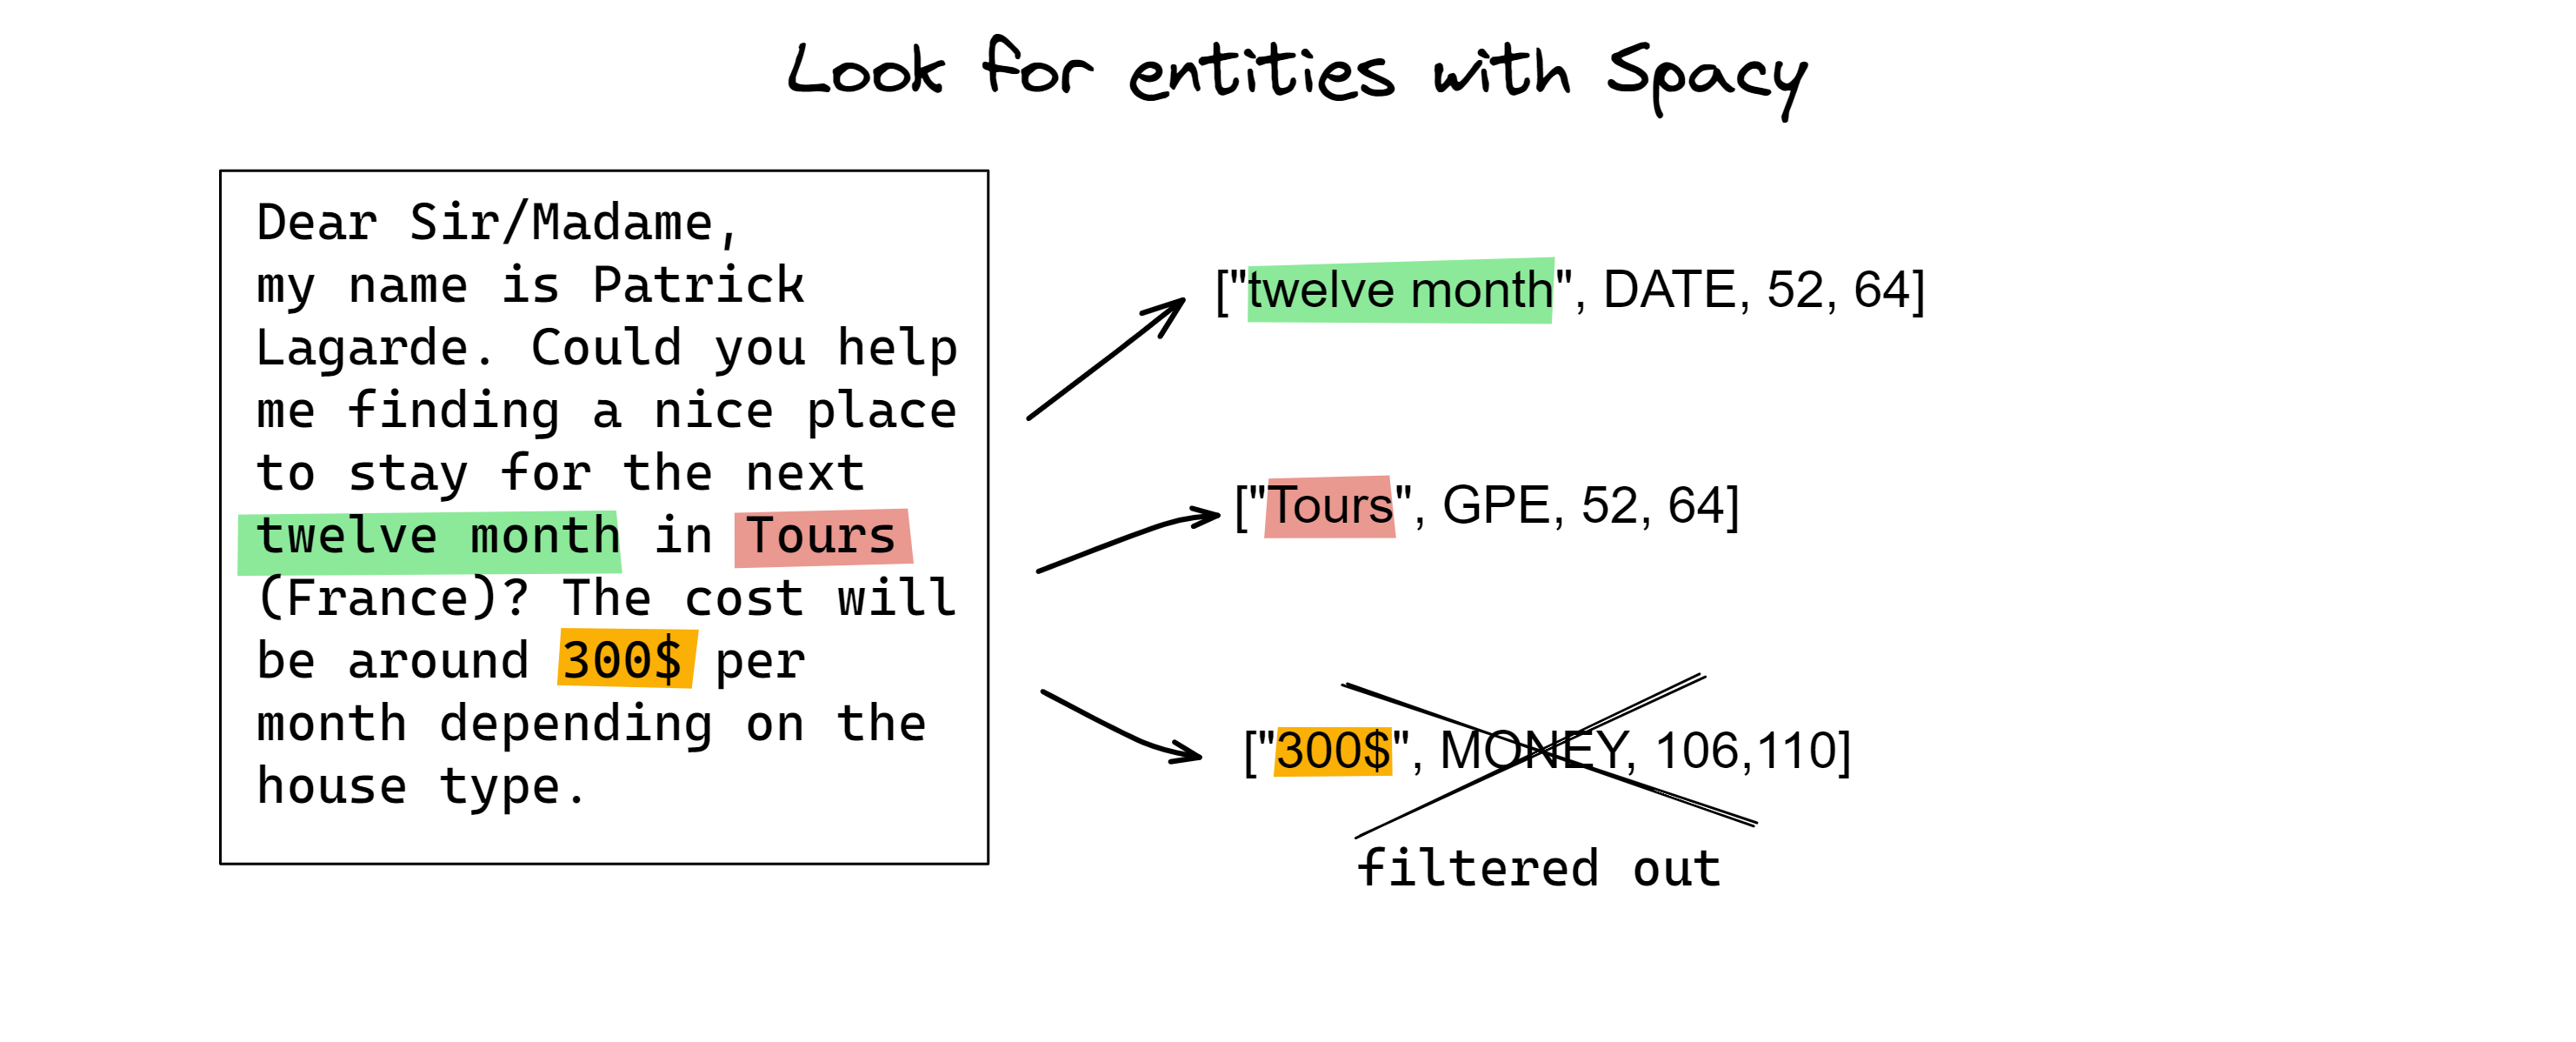
\includegraphics[width=\textwidth]{images/NER_nc_1.png}
    \caption{Ticket NER preprocessing part 1}
    \label{fig:ticket_NER_NC_1}
\end{figure}    
After that, we tokenize the text of all the tickets and we look up for each ticket its entities' tokens. Then for each entity, we save the indexes of the corresponding tokens, so for example if the entity "twelve months" is split into two tokens "twelve" and "month", which are the $22^{nd}$ and $23^{rd}$ tokens of the text, then we will save ["twelve months", DATE, [22,23]]. \\
We also had to manage the case in which a token is not present in the tokenizer vocabulary, so is split into sub-tokens. We took advantage of the fact that if a word is split into two or more words the new tokens will have the prefix "\#\#". \\
The number of tokens for each entity can vary, for practical reasons in the training phase we set the maximum number of tokens to $N=50$ (\autoref{fig:ticket_NER_NC_2}).
\begin{figure}[h] 
    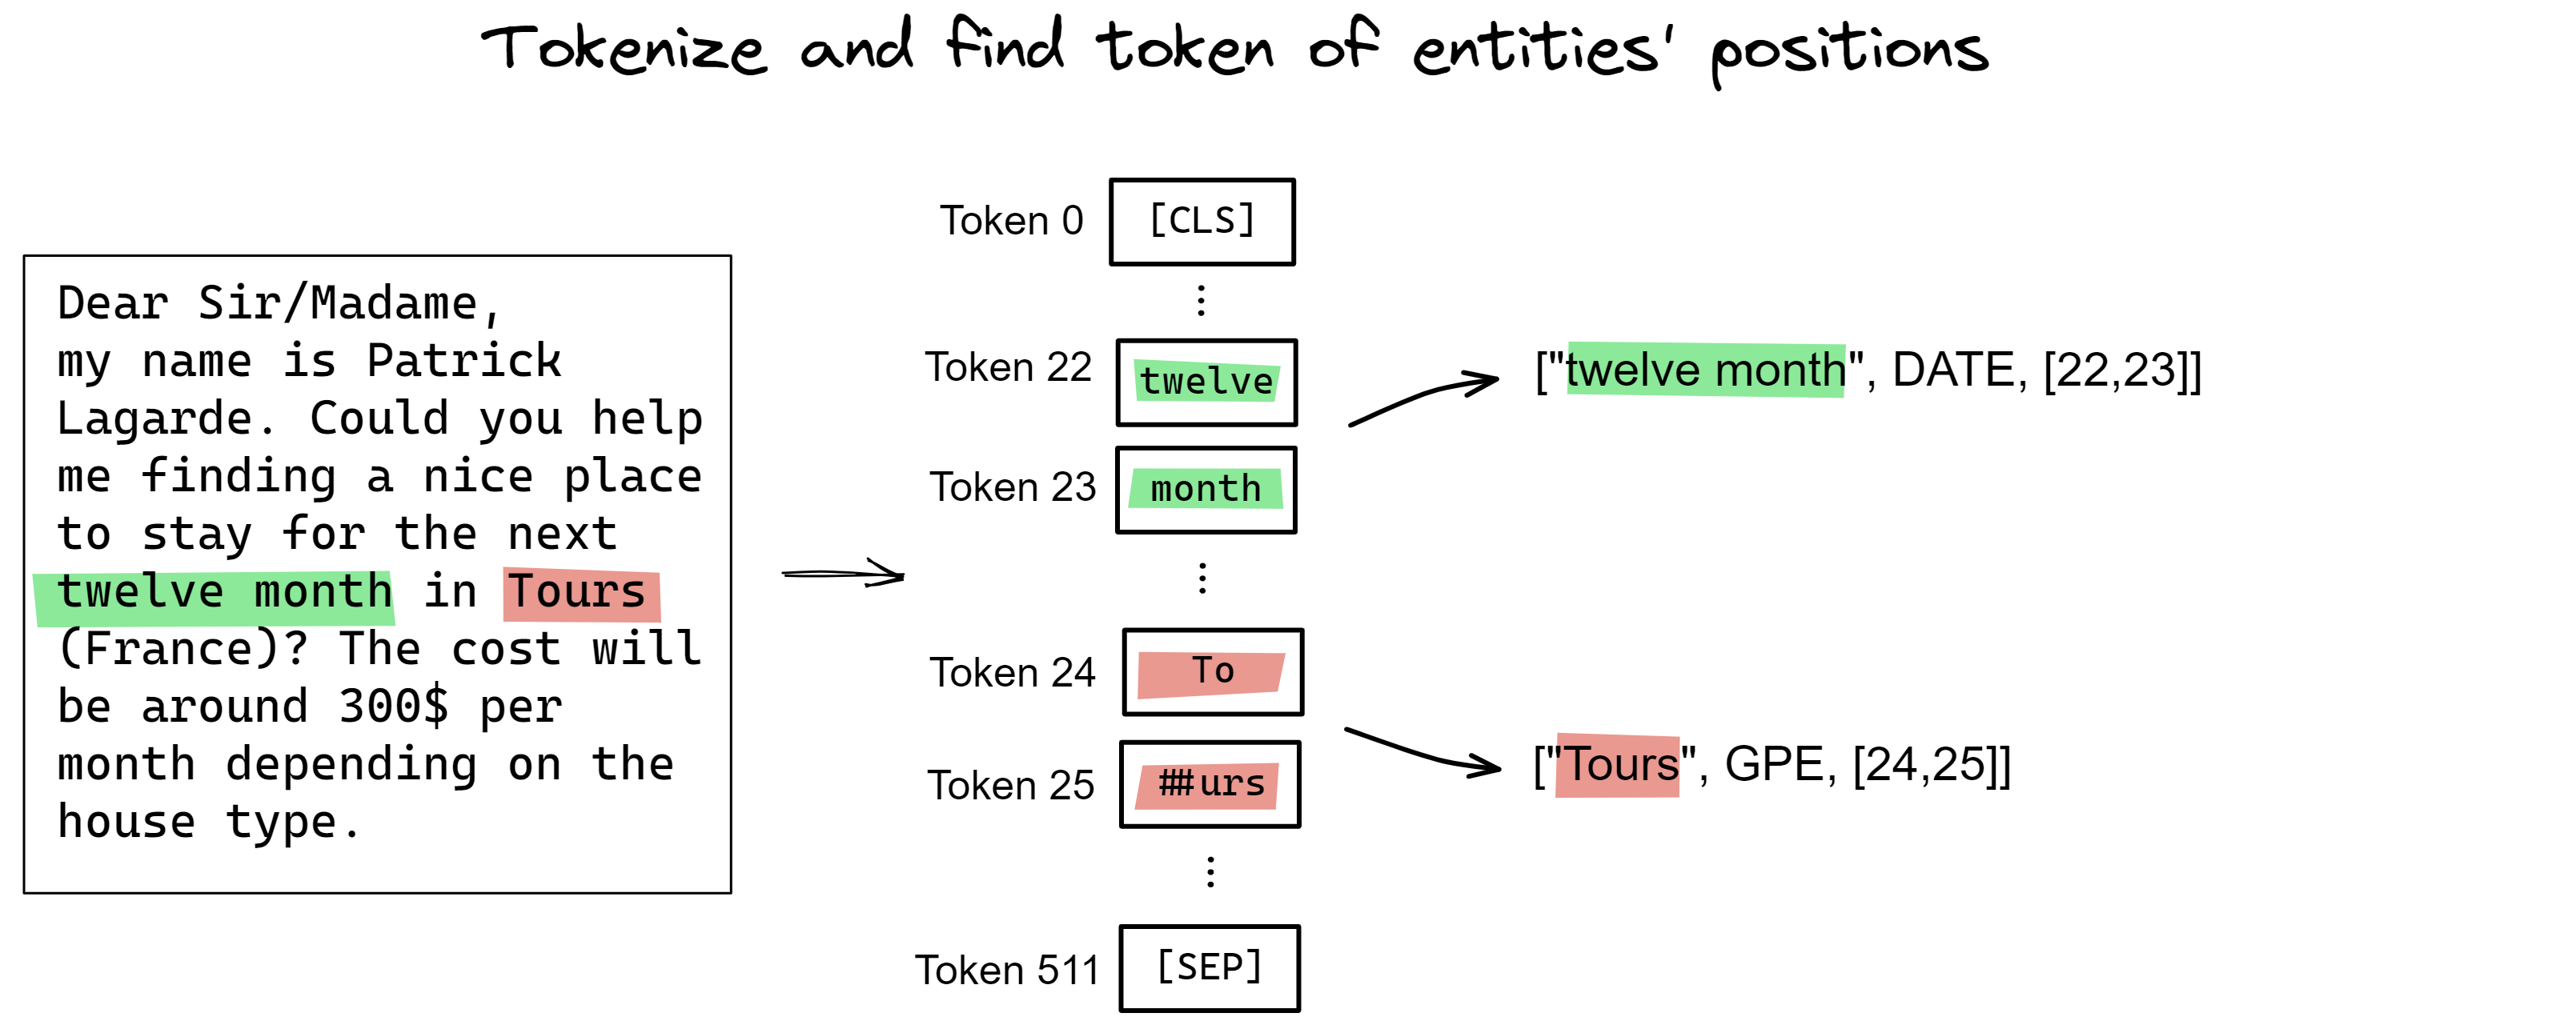
\includegraphics[width=\textwidth]{images/NER_nc_2.png}
    \caption{Ticket NER preprocessing part 2}
    \label{fig:ticket_NER_NC_2}
\end{figure}    
Now we have all we need for the training. The base architecture is a \textit{bert-base-cased} model, which we modified on the last layer. \\
In the training phase, we pass to the BERT model at each step the tickets' texts and their entities with the indexes of the matching tokens. For each entity of the ticket, there will be a training record. The ticket will be unpacked into 512 tokens, and each token will be processed by the BERT architecture (same architecture as the classifier \autoref{fig:bert_class}). \\
At the last layer, instead of passing the [CLS] token to a classifier, we concatenate the [CLS] token with the average of all the embeddings of the tokens of the current entity. This is the reason why we preprocessed the dataset to find the indexes of the tokens' indexes for the entities. In BERT base each token has a dimension $d=768$, so the input of the last feed forward neural network will be $N=1536$. The output dimension will be $M=10$ (\autoref{fig:ticket_NER_NC_3}). The labels of the training are the combination of the ticket category and the entity, since for each entity found in a ticket we generate a record ( For example if there are 3 entities in a ticket, there will be 3 records in the training set with the same ticket text, but that will have a different token embedding for the classification in the last layer and they will have different labels)\\
\begin{figure}[h] 
    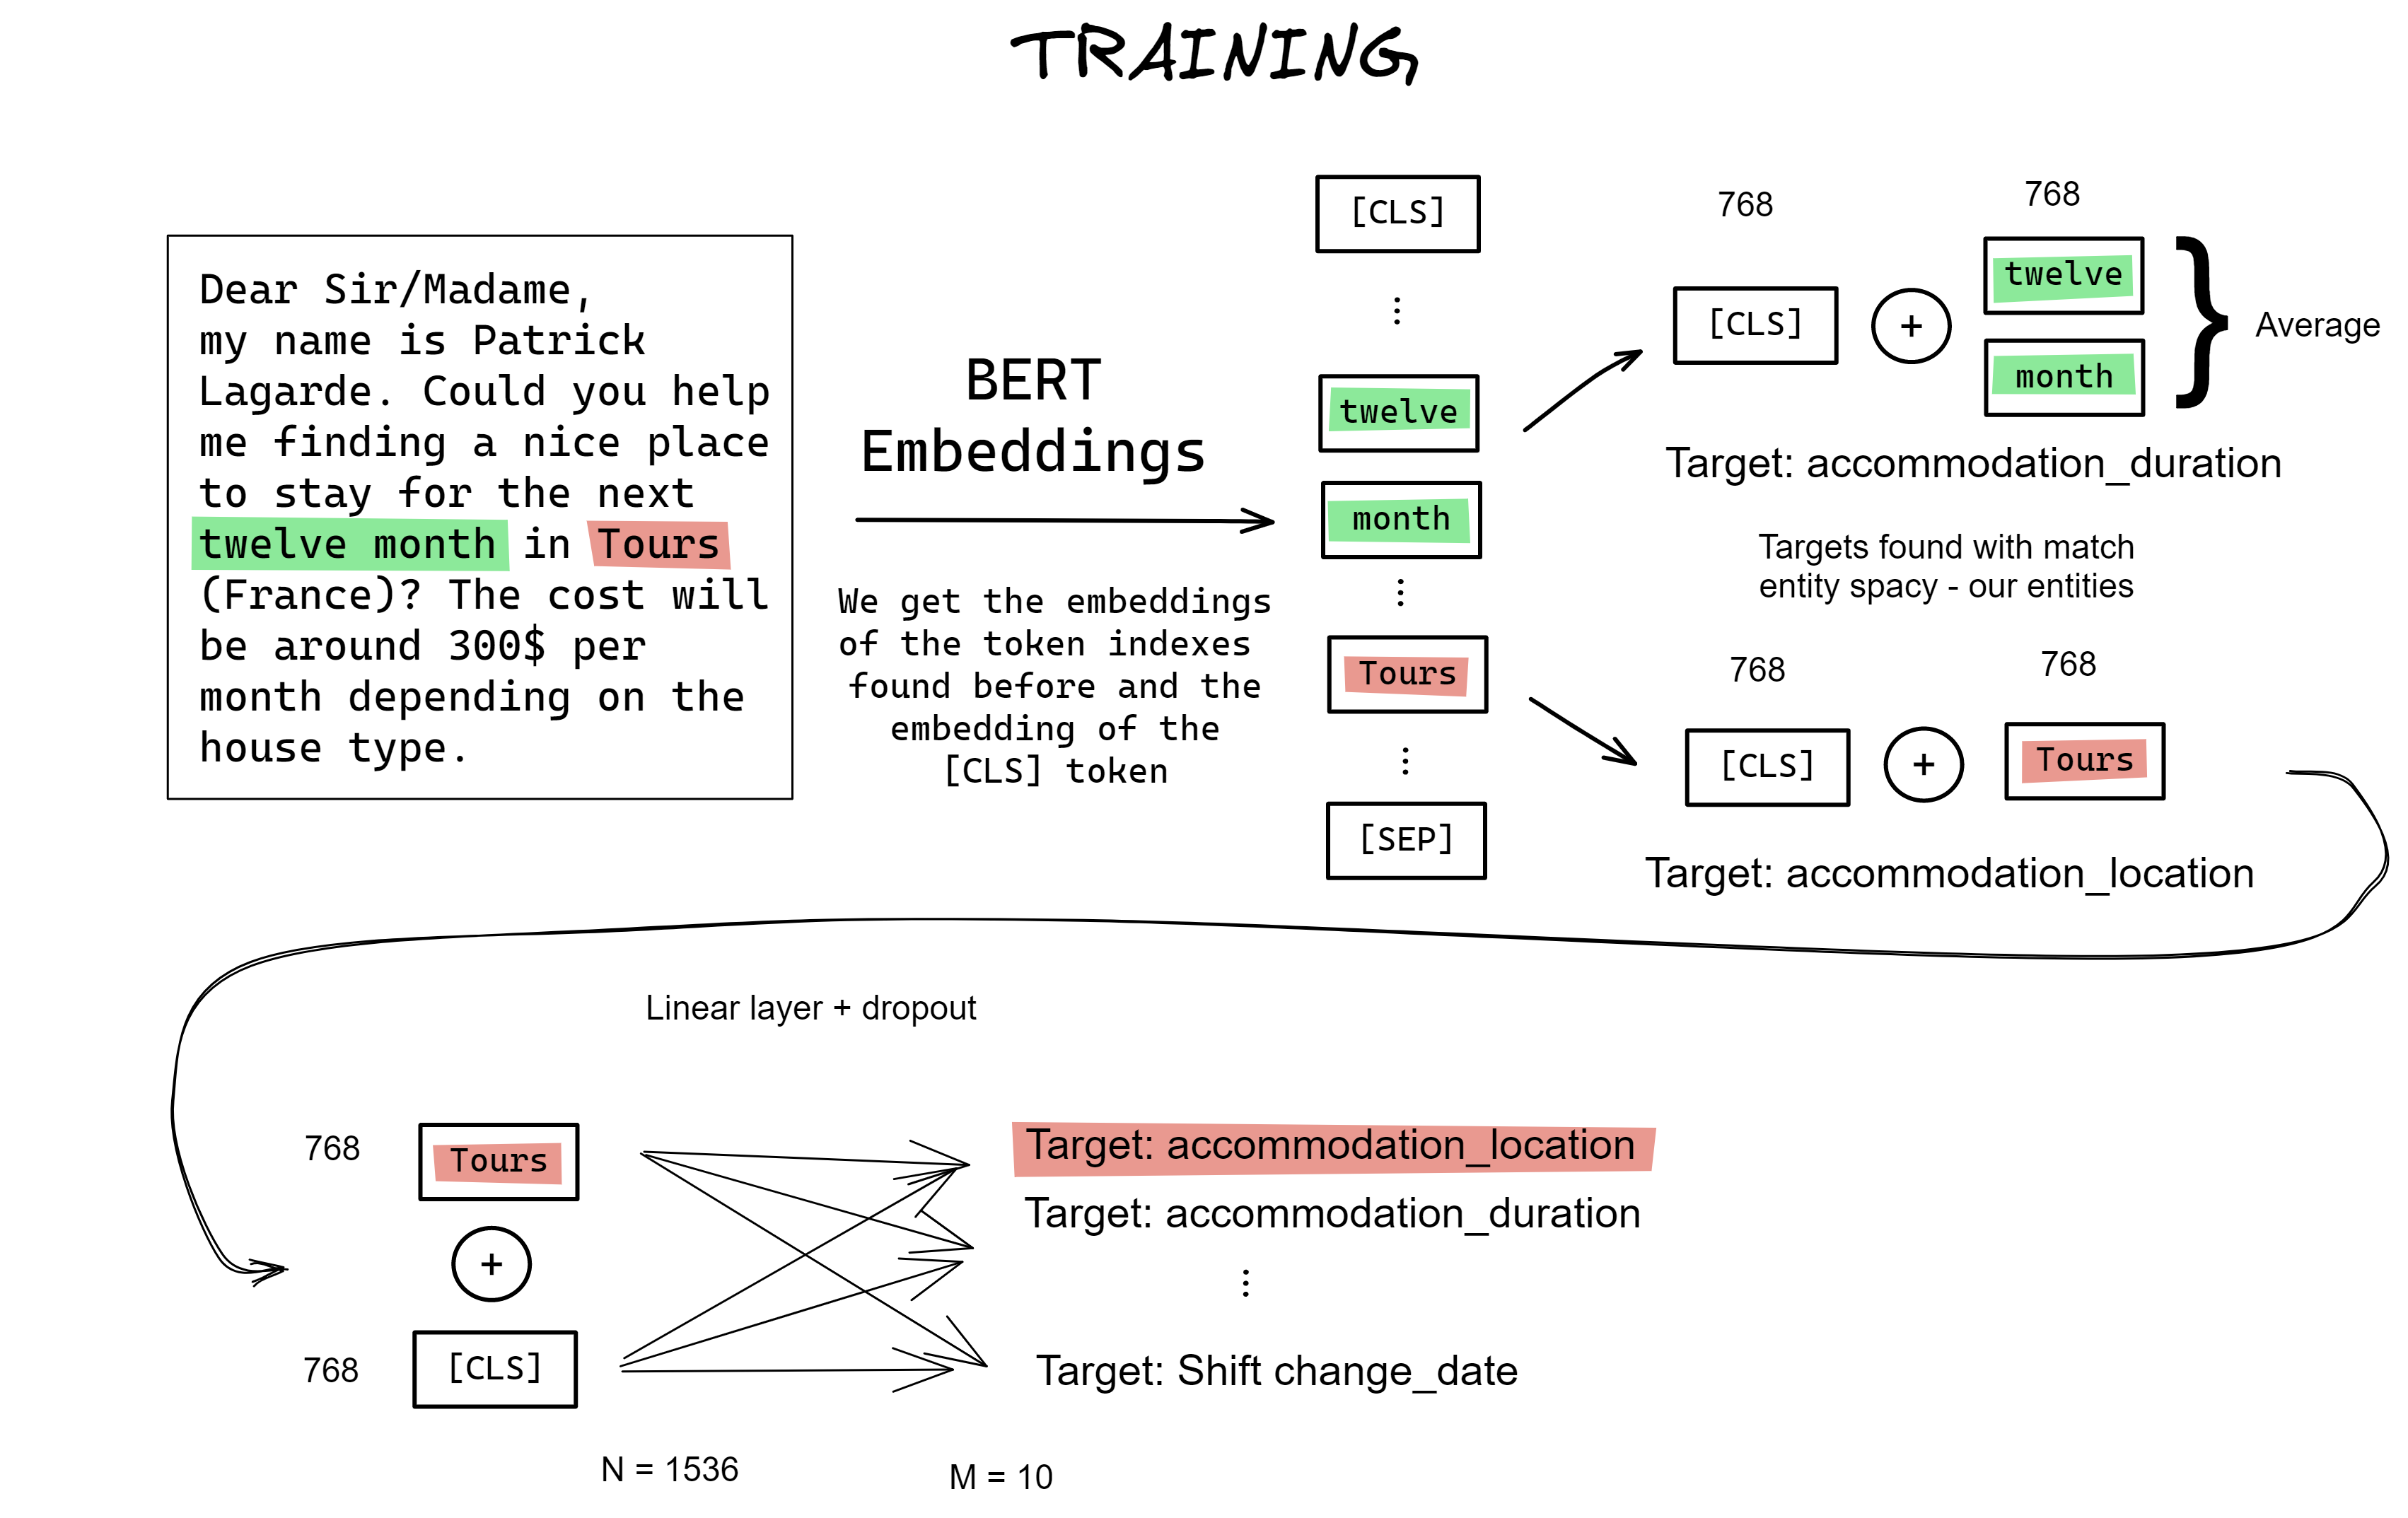
\includegraphics[width=\textwidth]{images/NER_nc_3.png}
    \caption{Ticket NER training}
    \label{fig:ticket_NER_NC_3}
\end{figure}
At test time, for each ticket in the test set, we analyze it with Spacy and we find all the entities. Then we filter the entities: we cannot filter based on the label, since at test time in theory we do not know the label of the tickets. Therefore we filter the entities based on the list of all entities used in all tickets' categories. \\
Then, as in the training phase, for each entity we build a new record composed of the output of the [CLS] token through the model architecture and of the average of the tokens' embeddings. \\
For each ticket in the test set we obtain a prediction of its category combined with the entity currently analyzed. 
\subsubsection*{Results}
We are able to achieve way better results with the new method that combines a ticket classifier with a NER model. On the test set we achieve a $f_1$ score of 0.96. \\
In \autoref{fig:ticket_NER_NC_conf_matrix} we show the confusion matrix of the classification. \\
We believe that we are able to achieve such good results because there are few entities that are shared between more categories, and the union of the information of the ticket ([CLS] token) and the information of the entity makes it easy for the model to distinguish both the category and the entity.
\begin{figure}[h] 
    \centering
    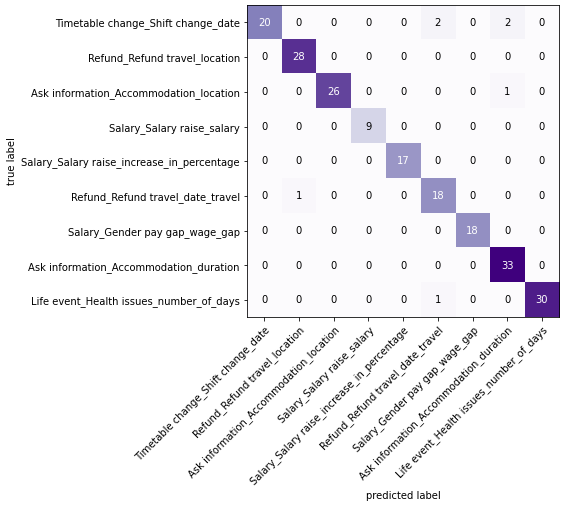
\includegraphics[width=0.8\textwidth]{images/conf_matrix_ner_nc.png}
    \caption{Ticket NER confusion matrix}
    \label{fig:ticket_NER_NC_conf_matrix}
\end{figure}   
